\documentclass[fontsize=12pt, titlepage, bibliography=totoc, listof=totoc]{scrartcl}
\usepackage[T1]{fontenc}
\usepackage[utf8]{inputenc}
\usepackage[english]{babel}
\usepackage[autostyle]{csquotes}
\usepackage{multirow}
\usepackage{graphicx}
\usepackage{amsmath}
\usepackage{longtable}
\usepackage{hyperref}
\usepackage{lmodern}
\usepackage{float}
\usepackage{cite}
\usepackage{subcaption}

\graphicspath{ {./figures/} }

\begin{document}
%%%%%%%%%%%%%%%%%%%%%%%%%%%%%%%%%%%%%%%%%%%%%%%%%%%%%%%%%%%%%%%%%%%%%%%%%%%%%%%%
%Title
\author{Christian Ertler, Georg Krispel, Bernhard Rapp}
\title{Cell Boundary Detection using Random Forests}
\subject{Medical Image Analysis, Design Practical}

\maketitle
\tableofcontents

%%%%%%%%%%%%%%%%%%%%%%%%%%%%%%%%%%%%%%%%%%%%%%%%%%%%%%%%%%%%%%%%%%%%%%%%%%%%%%%%

%\section{Examples}
\label{sec:examples}

Lorem ipsum dolor sit amet, consetetur sadipscing elitr, sed diam nonumy eirmod tempor invidunt ut labore et dolore magna aliquyam erat, sed diam voluptua. At vero eos et accusam et justo duo dolores et ea rebum. Stet clita kasd gubergren, no sea takimata sanctus est Lorem ipsum dolor sit amet. Lorem ipsum dolor sit amet, consetetur sadipscing elitr, sed diam nonumy eirmod tempor invidunt ut labore et dolore magna aliquyam erat, sed diam voluptua. At vero eos et accusam et justo duo dolores et ea rebum. Stet clita kasd gubergren, no sea takimata sanctus est Lorem ipsum dolor sit amet~\cite{example}.

\subsection{Table}
\label{subsec:table}

\begin{table}[htb!]
\centering
\begin{tabular}{|l|l|l|} \hline
\multicolumn{3}{|c|}{Schedulers} \\ \hline
\multirow{3}{*}{Immediate} & RR & Round Robin \\
& EF & Earliest First \\
& LL & Lightest Loaded \\ \hline
\multirow{4}{*}{Batch} & MM & Min-Min \\ 
& MX & Max-Min \\
& DL & Dynamic Level \\ 
& RC & Relative Cost \\ \hline
\multirow{4}{*}{Evolutionary} & PN & This paper \\
& ZO & Genetic Algorithm\\
& TA & Tabu search\\
& SA & Simlulated Annealing \\ \hline
\end{tabular} \caption{Beispiel Tabelle}
\end{table}\label{tab:table}

\subsection{Figure}
\label{subsec:figure}

\subsubsection{Single Figure}
\label{subsubsec:single_figure}

\begin{figure}[H]
  \caption{Example picture}
  \centering
    \includegraphics[width=0.5\textwidth]{example}
\end{figure}

\subsubsection{Two Figures Side-by-Side}
\label{subsubsec:two_Figures}

\begin{figure}[h]
\begin{subfigure}{0.48\textwidth}
\includegraphics[width=\textwidth]{left_image}
\caption{First Figure}
\end{subfigure} \hspace{0.04\textwidth}
\begin{subfigure}{0.48\textwidth}
\includegraphics[width=\textwidth]{right_image}
\caption{Second Figure}
\end{subfigure}
\caption{Caption of both Figures}
\end{figure}

%\begin{figure}[H]
%\begin{minipage}[b]{0.45\linewidth}
%\centering
%\includegraphics[width=\textwidth]{left_image}
%\caption{First Figure}
%\label{fig:figure1}
%\end{minipage}
%\hspace{0.5cm}
%\begin{minipage}[b]{0.45\linewidth}
%\centering
%\includegraphics[width=\textwidth]{right_image}
%\caption{Second Figure}
%\label{fig:figure2}
%\end{minipage}
%\caption{Caption of both Figures}
%\end{figure}

\section{Objective}
\label{sec:objective}

The goal of this work is the detection of cell boundaries from electron microscopy images\footnote{\label{foot:1} \url{http://brainiac2.mit.edu/isbi_challenge/}}. Given are 30 labeled training images which should be used to train a random forest. To validate the performance of the implementation cross-validation should be done.
After training, an image should be processed by a sliding window which is moved over the entire image and classified by the forest.
Furthermore OpenCV\footnote{\label{foot:2} \url{http://opencv.org/}} for image processing and OpenMP \footnote{\label{foot:3} \url{http://openmp.org/wp/}} for parallelization should be used. CMake \footnote{\label{foot:4} \url{http://www.cmake.org/}} was used ensure a platform independent setup.

\section{Implementation}
\label{sec:implementation}
\section{Results}
\label{sec:results}

In this section, the result of our experiments with the forest will be evaluated. There are many parameters
of the forest which can be evaluated:

\FloatBarrier
\begin{enumerate}
	\item The number of training samples
	\item The patch size of the training samples
	\item The number of trees in the forest
	\item The maximal depth of each tree
	\item The minimum number of samples at which a node will be splitted again
	\item The number of random features to select at each node split
	\item Is bagging enabled?
\end{enumerate}
\FloatBarrier

To speed up the evaluation phase we decided to fixate most of the parameters and test different combinations
of the third, forth and sixth parameter. The setup looks as follows:

\FloatBarrier
\begin{description}
	\item[number of training samples:] 10000 per training images
	\item[patch size:] $30 \times 30$ pixels
	\item[number of trees:] 10, 20, 30, 40, 50
	\item[maximal depth:] 10, 11, 12, 13, 14, 15
	\item[minimum number of samples per node:] 10
	\item[number of random features:] 100, 150
	\item[bagging:] enabled
\end{description}
\FloatBarrier

The combination of the parameters gives us 60 different tests. The accuracy results of these tests can be seen
in figure \ref{fig:result_heatmap}. The first row shows the results of the cross validation. The results
of directly comparing the groundtruth image to the output of the forest are located in the second row. 

The plots show that the cross validation accuracy gets better by increasing any of the three varying parameters.
However, we expect the classifier to overfit for even larger depths and higher number of feature tests. The best
accuracy of $\approx 86.5\%$ was found for 50 trees, a depth of 15 and 150 feature tests per node. The image based
accuracy in the second row does not entirely reflect this result. This accuracy amounts to $\approx 79.6\%$ whereas
the best value is at $\approx 79.9\%$.

It is also interesting to see, that the number of trees has a negligible impact on the cross validation accuracy.
For the image based accuracy on the other hand, the impact is higher.


\begin{figure}
	\centering
	\begin{subfigure}{0.4\textwidth}
		\centering
		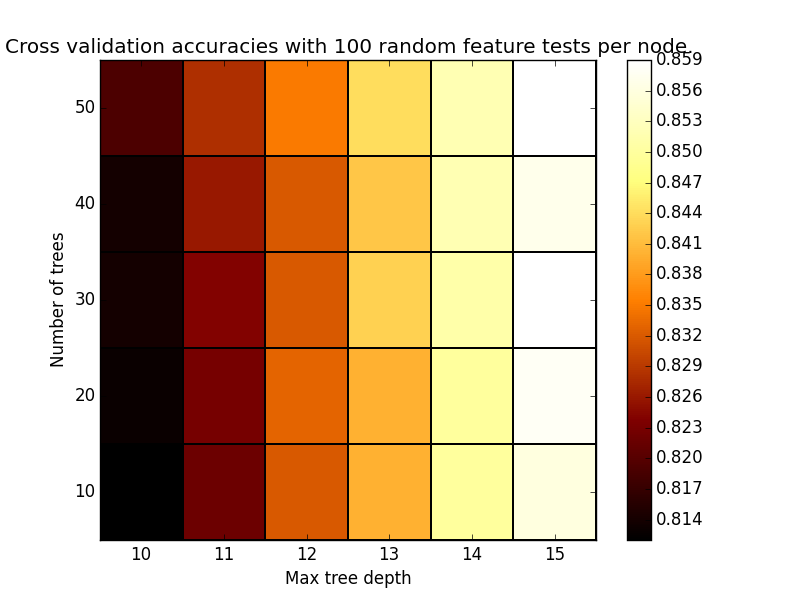
\includegraphics[width=\textwidth]{plots/heatmap_xacc_100.png}
		\caption{Cross validation accuracies. (100 features per node)}
		\label{subfig:result_heatmap_xacc_100}
	\end{subfigure}
	\begin{subfigure}{0.4\textwidth}
		\centering
		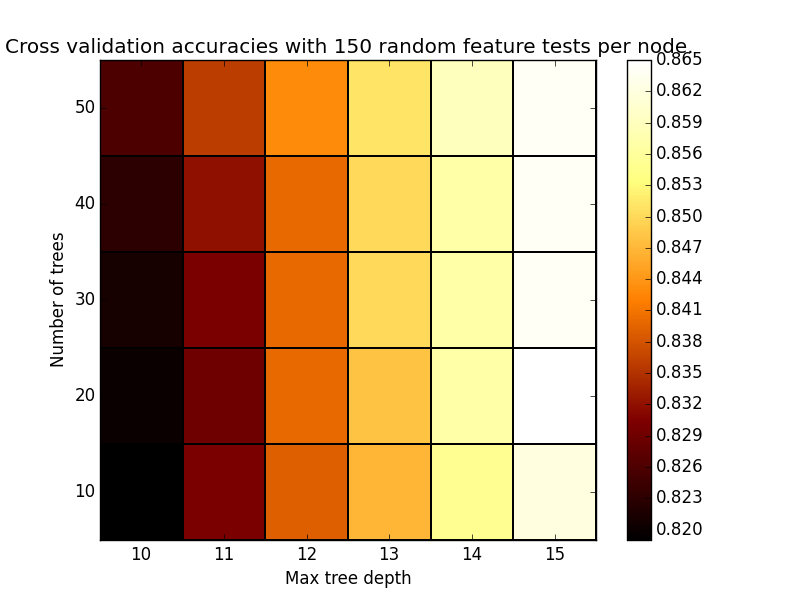
\includegraphics[width=\textwidth]{plots/heatmap_xacc_150.png}
		\caption{Cross validation accuracies. (150 features per node)}
		\label{subfig:result_heatmap_xacc_150}
	\end{subfigure}

	\begin{subfigure}{0.4\textwidth}
		\centering
		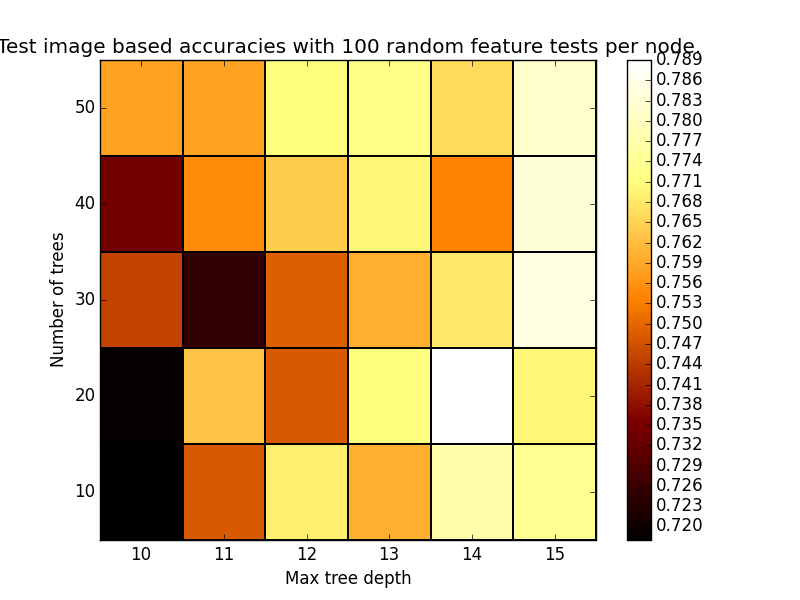
\includegraphics[width=\textwidth]{plots/heatmap_iacc_100.png}
		\caption{Accuracies based on groundtruth images. (100 features per node)}
		\label{subfig:result_heatmap_iacc_100}
	\end{subfigure}
	\begin{subfigure}{0.4\textwidth}
		\centering
		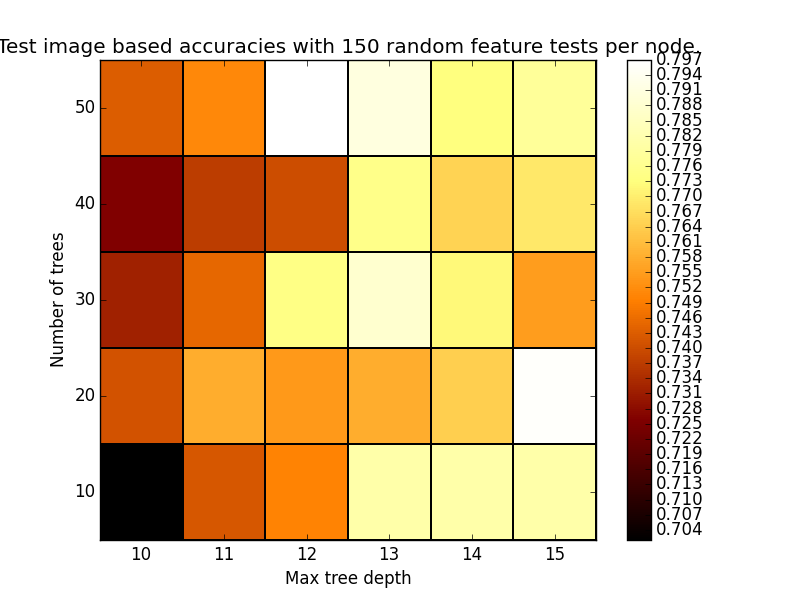
\includegraphics[width=\textwidth]{plots/heatmap_iacc_150.png}
		\caption{Accuracies based on groundtruth images. (150 features per node)}
		\label{subfig:result_heatmap_iacc_150}
	\end{subfigure}
	\caption{Accuracy results.}
	\label{fig:result_heatmap}
\end{figure}

Figure \ref{fig:result_images_best_xacc} shows the output images corresponding to
the forest with the best cross validation accuracy ($\approx 86.5\%$) and figure
\ref{fig:result_images_best_iacc} those corresponding to the forest with the best
accuracy on the test image ($\approx 79.9\%$). From a human point of view the latter
looks better.

\begin{figure}
	\centering
	\begin{subfigure}[t]{0.3\textwidth}
		\centering
		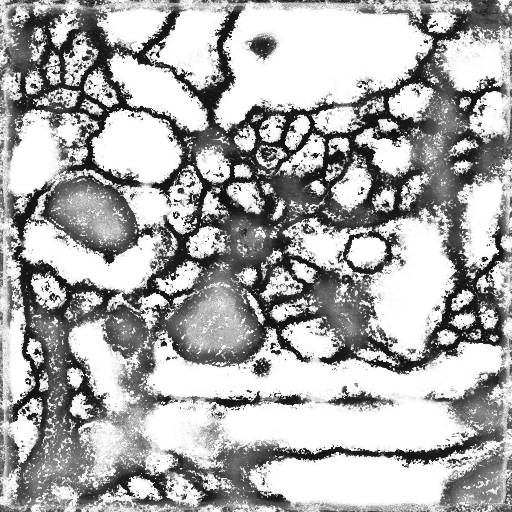
\includegraphics[width=\textwidth]{{{images/0.865-1435707507-0021-prop}}}
		\caption{Forest probabilities}
	\end{subfigure}
	\begin{subfigure}[t]{0.3\textwidth}
		\centering
		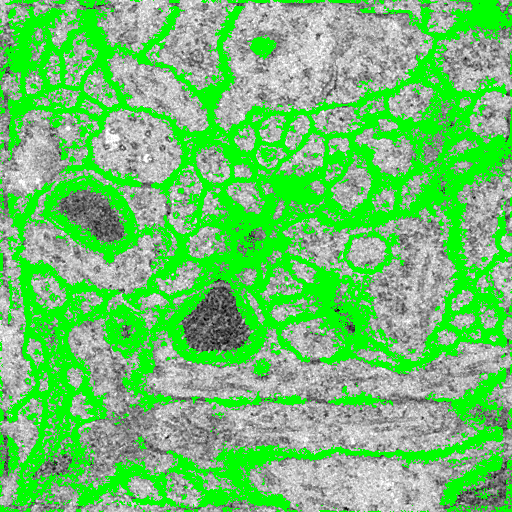
\includegraphics[width=\textwidth]{{{images/0.865-1435707507-0021-overlay}}}
		\caption{Predictions}
	\end{subfigure}
	\begin{subfigure}[t]{0.3\textwidth}
		\centering
		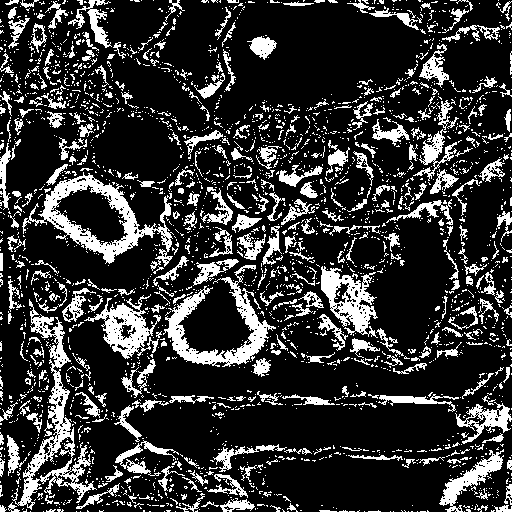
\includegraphics[width=\textwidth]{{{images/0.865-1435707507-0021-diff}}}
		\caption{Absolute difference to the ground truth}
	\end{subfigure}
	\caption{Forest outputs with 50 trees, depth 15 and 150 feature tests.}
	\label{fig:result_images_best_xacc}
\end{figure}

\begin{figure}
	\centering
	\begin{subfigure}[t]{0.3\textwidth}
		\centering
		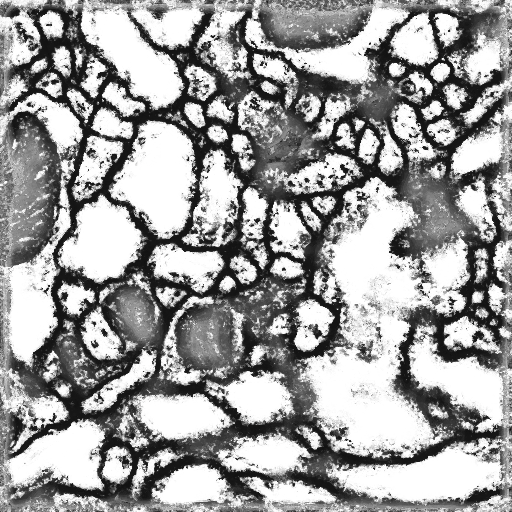
\includegraphics[width=\textwidth]{{{images/0.843-1435685565-0013-prop}}}
		\caption{Forest probabilities}
	\end{subfigure}
	\begin{subfigure}[t]{0.3\textwidth}
		\centering
		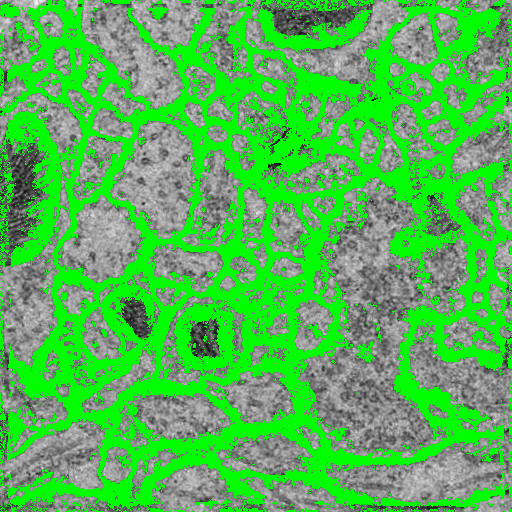
\includegraphics[width=\textwidth]{{{images/0.843-1435685565-0013-overlay}}}
		\caption{Predictions}
	\end{subfigure}
	\begin{subfigure}[t]{0.3\textwidth}
		\centering
		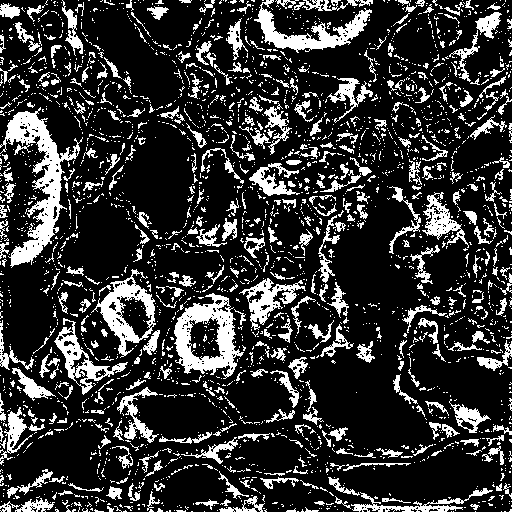
\includegraphics[width=\textwidth]{{{images/0.843-1435685565-0013-diff}}}
		\caption{Absolute difference to the ground truth}
	\end{subfigure}
	\caption{Forest outputs with 10 trees, depth 12 and 150 feature tests.}
	\label{fig:result_images_best_iacc}
\end{figure}

The simple distinction between border and cell pixels works quite well though the forest
tends to classify near-border pixels as borders as well. Most of the differences to the
ground truth are due to those misclassifications. As we can see in the output probabilities,
the forest is also able to distinguish between border and nucleus pixels. However, it tends
to classify the borders of the nucleuses as cell borders which is not optimal. 
\section{Conclusion}
\label{sec:conclusion}
\newpage

\bibliography{bibliography}{}
\bibliographystyle{plain}
\end{document}
